\documentclass[12pt,a4paper]{report}
\usepackage[spanish,es-tabla]{babel}
\usepackage[utf8]{inputenc}
\usepackage[T1]{fontenc}
\usepackage{geometry}
\usepackage{graphicx}
\usepackage{caption}
\usepackage{subcaption}
\usepackage{amsmath, amssymb}
\usepackage{siunitx}
\usepackage{hyperref}
\usepackage{xcolor}
\usepackage{listings}
\usepackage{float}
\geometry{margin=1in}
\hypersetup{colorlinks=true,linkcolor=blue,urlcolor=blue,citecolor=blue}

\definecolor{codebg}{RGB}{245,245,245}
\lstdefinestyle{mypython}{
  language=Python,
  basicstyle=\ttfamily\small,
  backgroundcolor=\color{codebg},
  frame=single,
  showstringspaces=false,
  keywordstyle=\color{blue!60!black},
  commentstyle=\color{green!40!black},
  stringstyle=\color{red!60!black},
  numbers=left,
  numberstyle=\tiny, 
  stepnumber=1,
  numbersep=8pt,
  tabsize=2,
  breaklines=true,
  keepspaces=true
}

\begin{document}

% Portada
\begin{titlepage}
  \centering
  {\Large Informe Académico}\par\vspace{0.75cm}
  {\LARGE Aplicación del Método de Newton–Raphson en la solución del sistema de ecuaciones no lineales\par}
  \vspace{0.75cm}
  {\large Basado en los archivos del repositorio, incl. `Introducción al sistema.pdf`}\par
  \vspace{1.25cm}
  {\large Autores (según `Introducción al sistema.pdf`):\par}
  \vspace{0.25cm}
  {\large Ervin Caravali Ibarra — 1925648\par}
  {\large Juan Esteban Ortiz Bejarano — 2410227\par}
  {\large Brayan Camilo Urrea Jurado — 2410023\par}
  \vfill
  {\large Fecha: \today}\par
\end{titlepage}

\tableofcontents
\clearpage

\chapter{Introducción}
Este informe documenta la implementación y presentación del método de Newton–Raphson aplicado a un sistema de ecuaciones no lineales discretizado sobre una malla de \(5\times 50\) nodos, con condiciones de borde y una viga interna que introduce nodos fijos/omitidos. La fuente visual principal es el documento `Introducción al sistema.pdf`, del cual se extraen figuras para ilustrar la formulación. La especificación detallada, el algoritmo y el código en Python provienen de `AVANCE 2.md` y `AVANCE 2.docx`.

\begin{figure}[H]
  \centering
  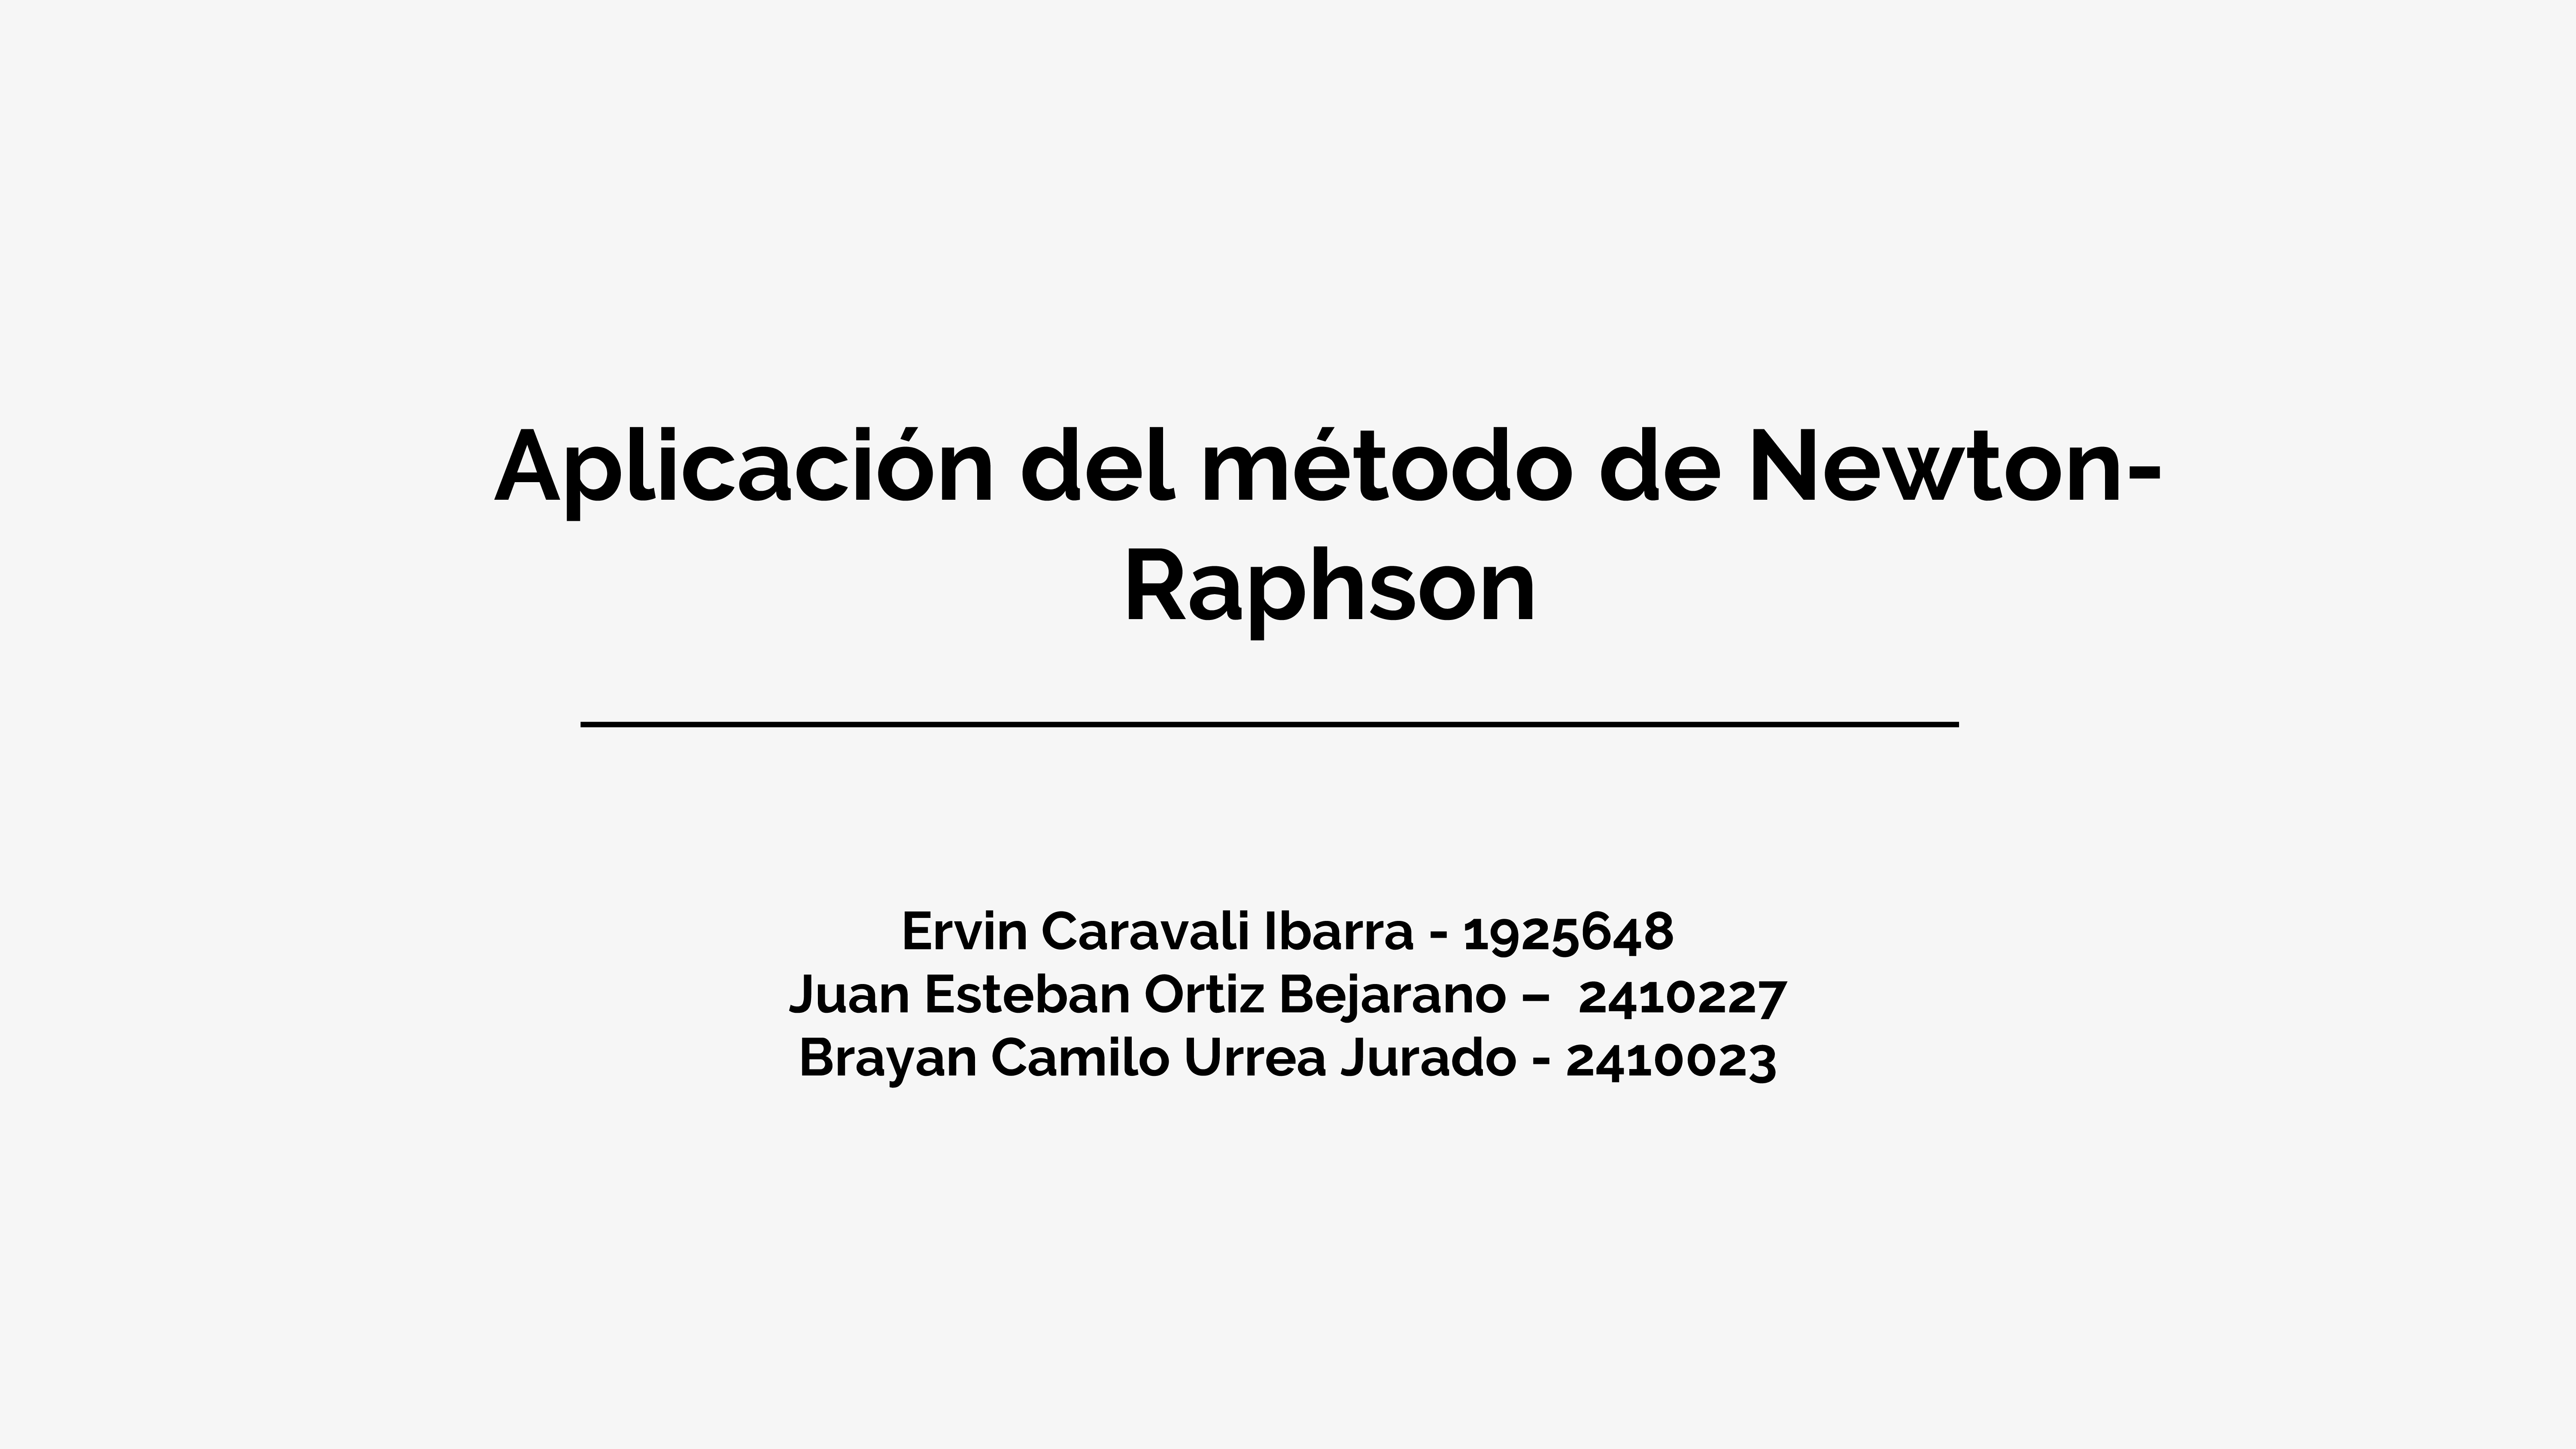
\includegraphics[width=0.95\textwidth]{intro_img-000.png}
  \caption{Portada y créditos (extraída de `Introducción al sistema.pdf`).}
\end{figure}

\chapter{Planteamiento del problema}
La dinámica sobre la malla se expresa en términos de la velocidad \(V\) en nodos discretos. El problema original se reescribe como una ecuación de equilibrio \(F(V)=0\), condición necesaria en el estado estacionario buscado.

\section{Vector de incógnitas y conteo}
La malla total tiene 250 nodos (\(5\) filas \(\times\) \(50\) columnas), pero no todos son incógnitas. Se excluyen las fronteras (valores fijos) y los \(10\) nodos de la viga, dando lugar a \(144-10=134\) incógnitas.

\begin{figure}[H]
  \centering
  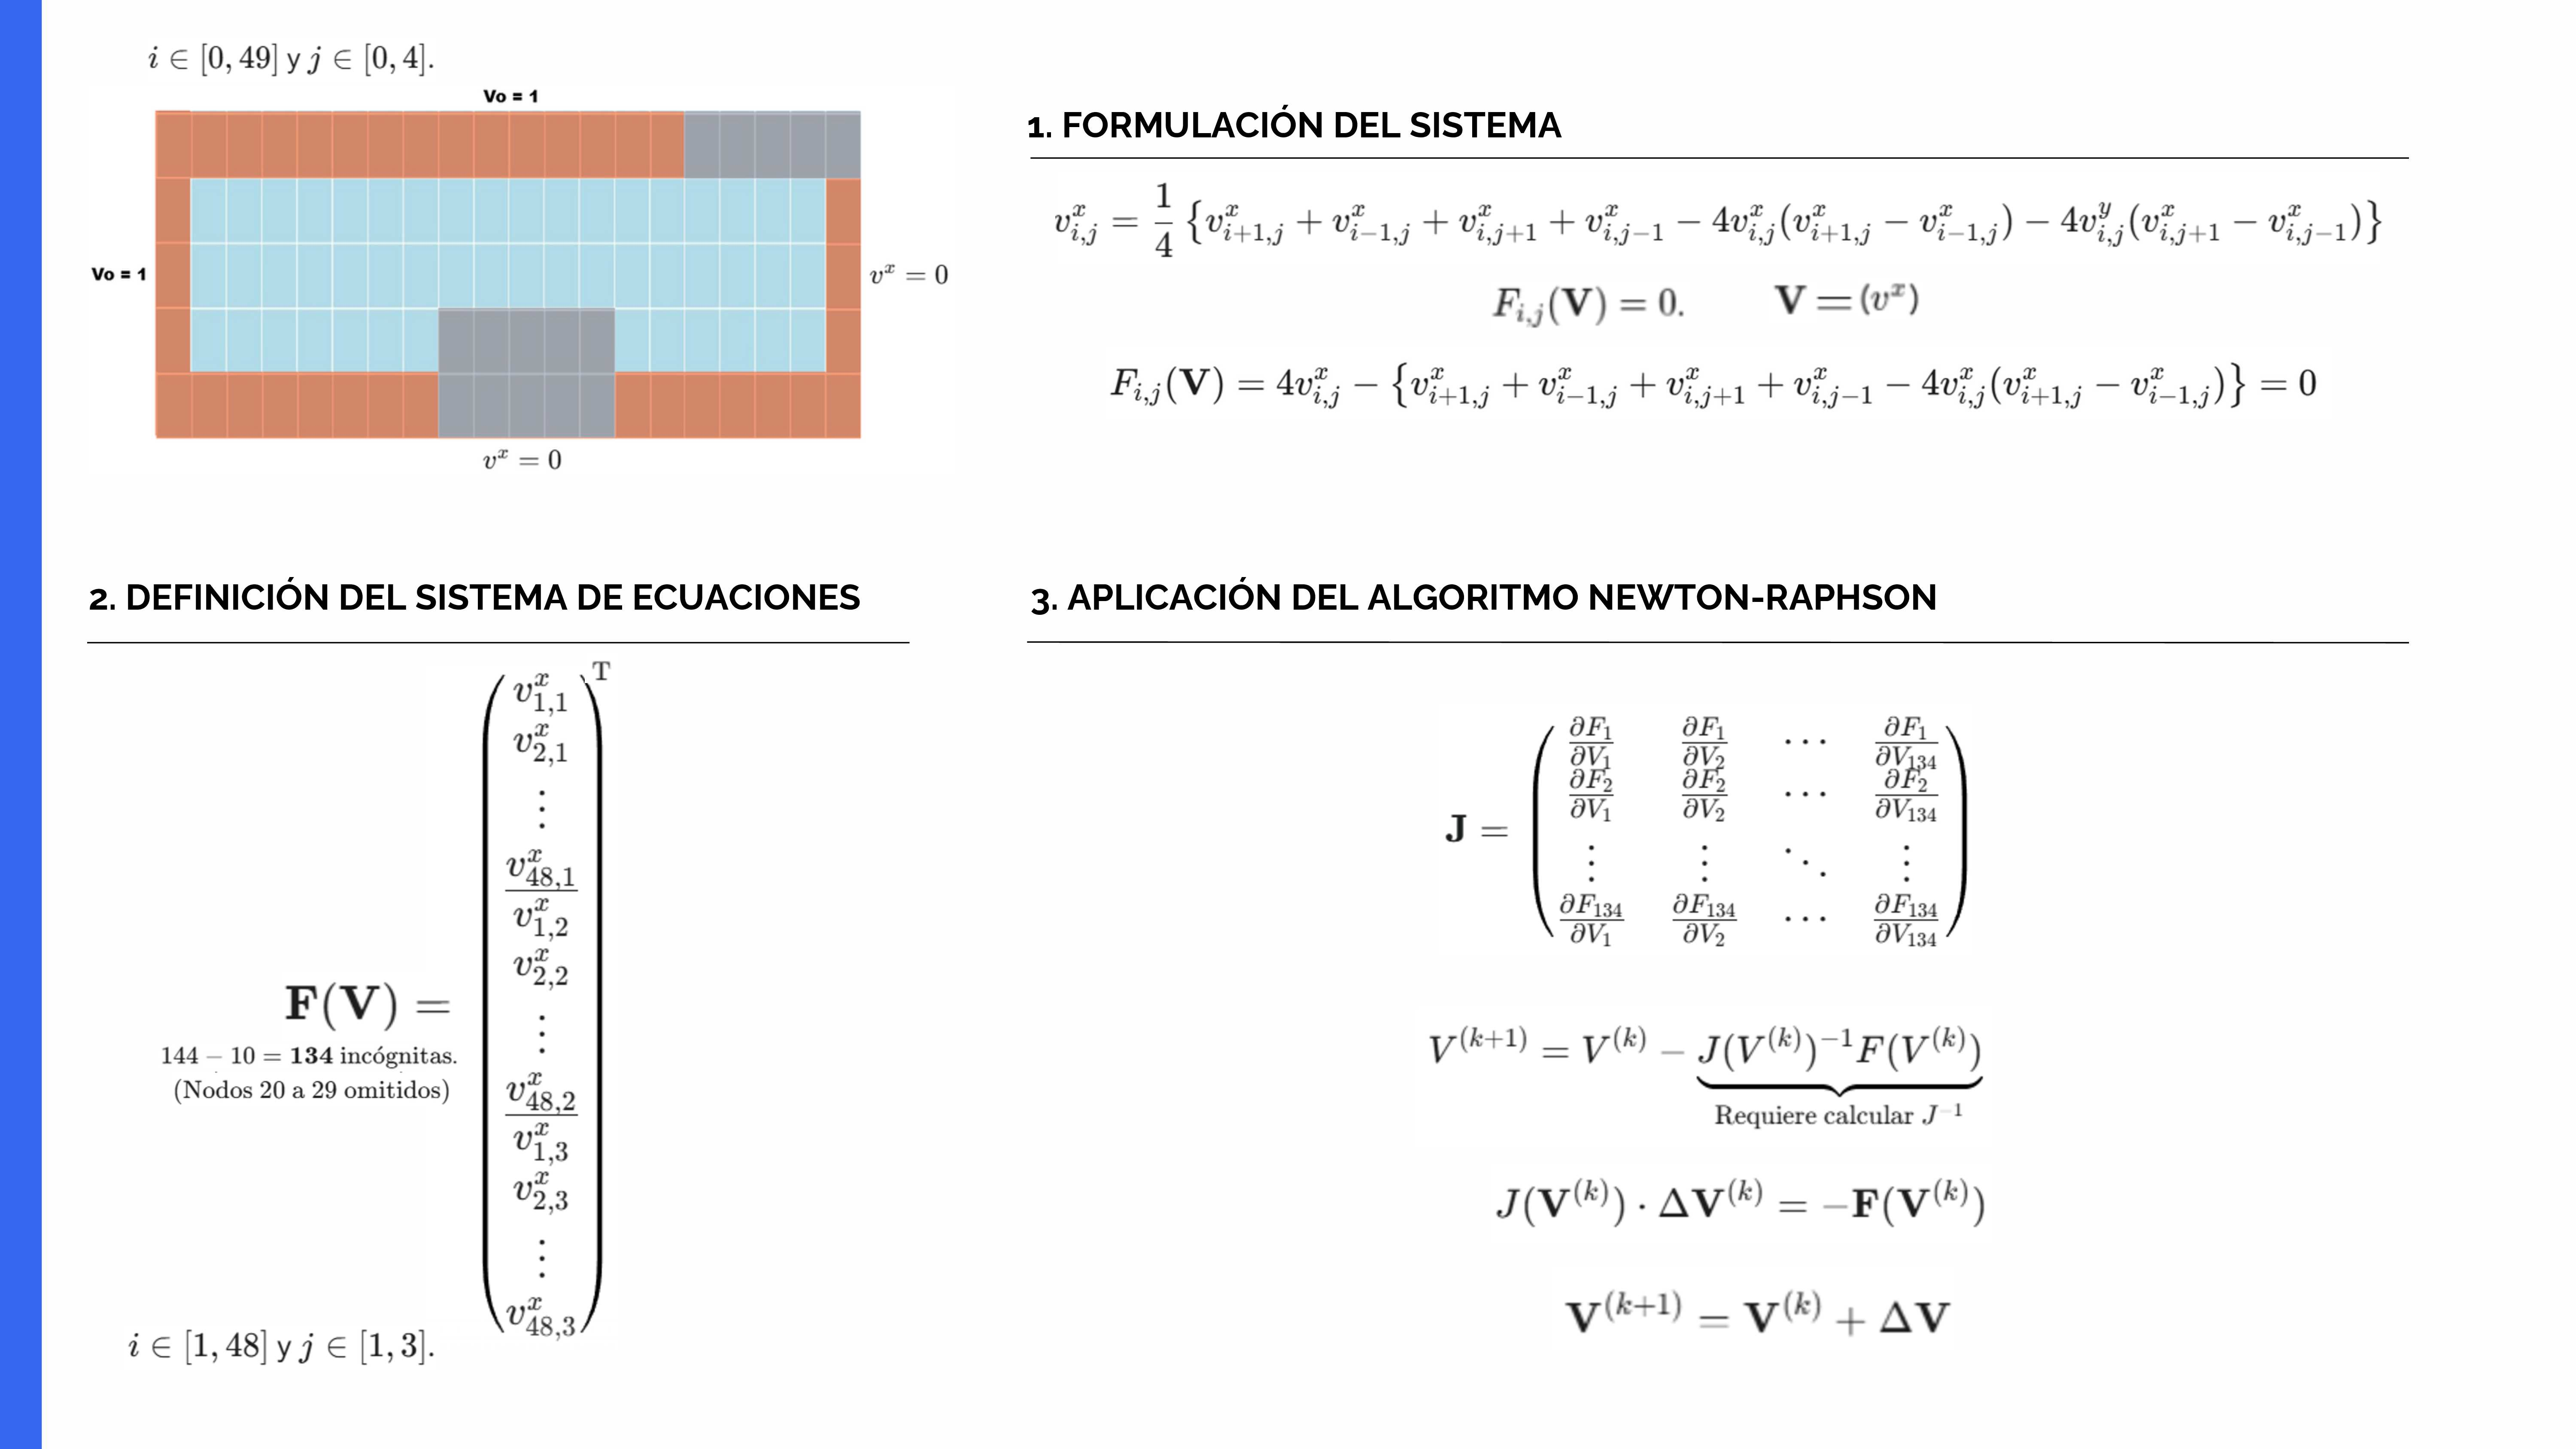
\includegraphics[width=0.95\textwidth]{intro_img-001.png}
  \caption{Formulación de \(F(V)\) y conteo de incógnitas (extraída de `Introducción al sistema.pdf`).}
\end{figure}

\chapter{Formulación del residual y Jacobiano}
\section{Residual no lineal}
Para cada nodo interior \((i,j)\), el residual \(F_m\) asociado a la incógnita \(V_{ij}\) (índice plano \(m\)) se plantea como
\[\small
F_m = 4\,V_{ij} - (V_{i+1,j}+V_{i-1,j}+V_{i,j+1}+V_{i,j-1}) 
      + c\,V_{ij}\,V_{i-1,j} - c\,V_{ij}\,V_{i+1,j},
\]
con \(c=\) FACTOR\_CONVECCION. Este \(F(V)=0\) reúne términos difusivos (laplaciano) y convectivos no lineales.

\section{Jacobiano}
Se ensambla la matriz jacobiana \(J=\partial F/\partial V\) considerando derivadas parciales respecto del nodo central y sus cuatro vecinos (derecha, izquierda, superior, inferior). Su estructura es esparsa y de tamaño \(134\times 134\).

\begin{figure}[H]
  \centering
  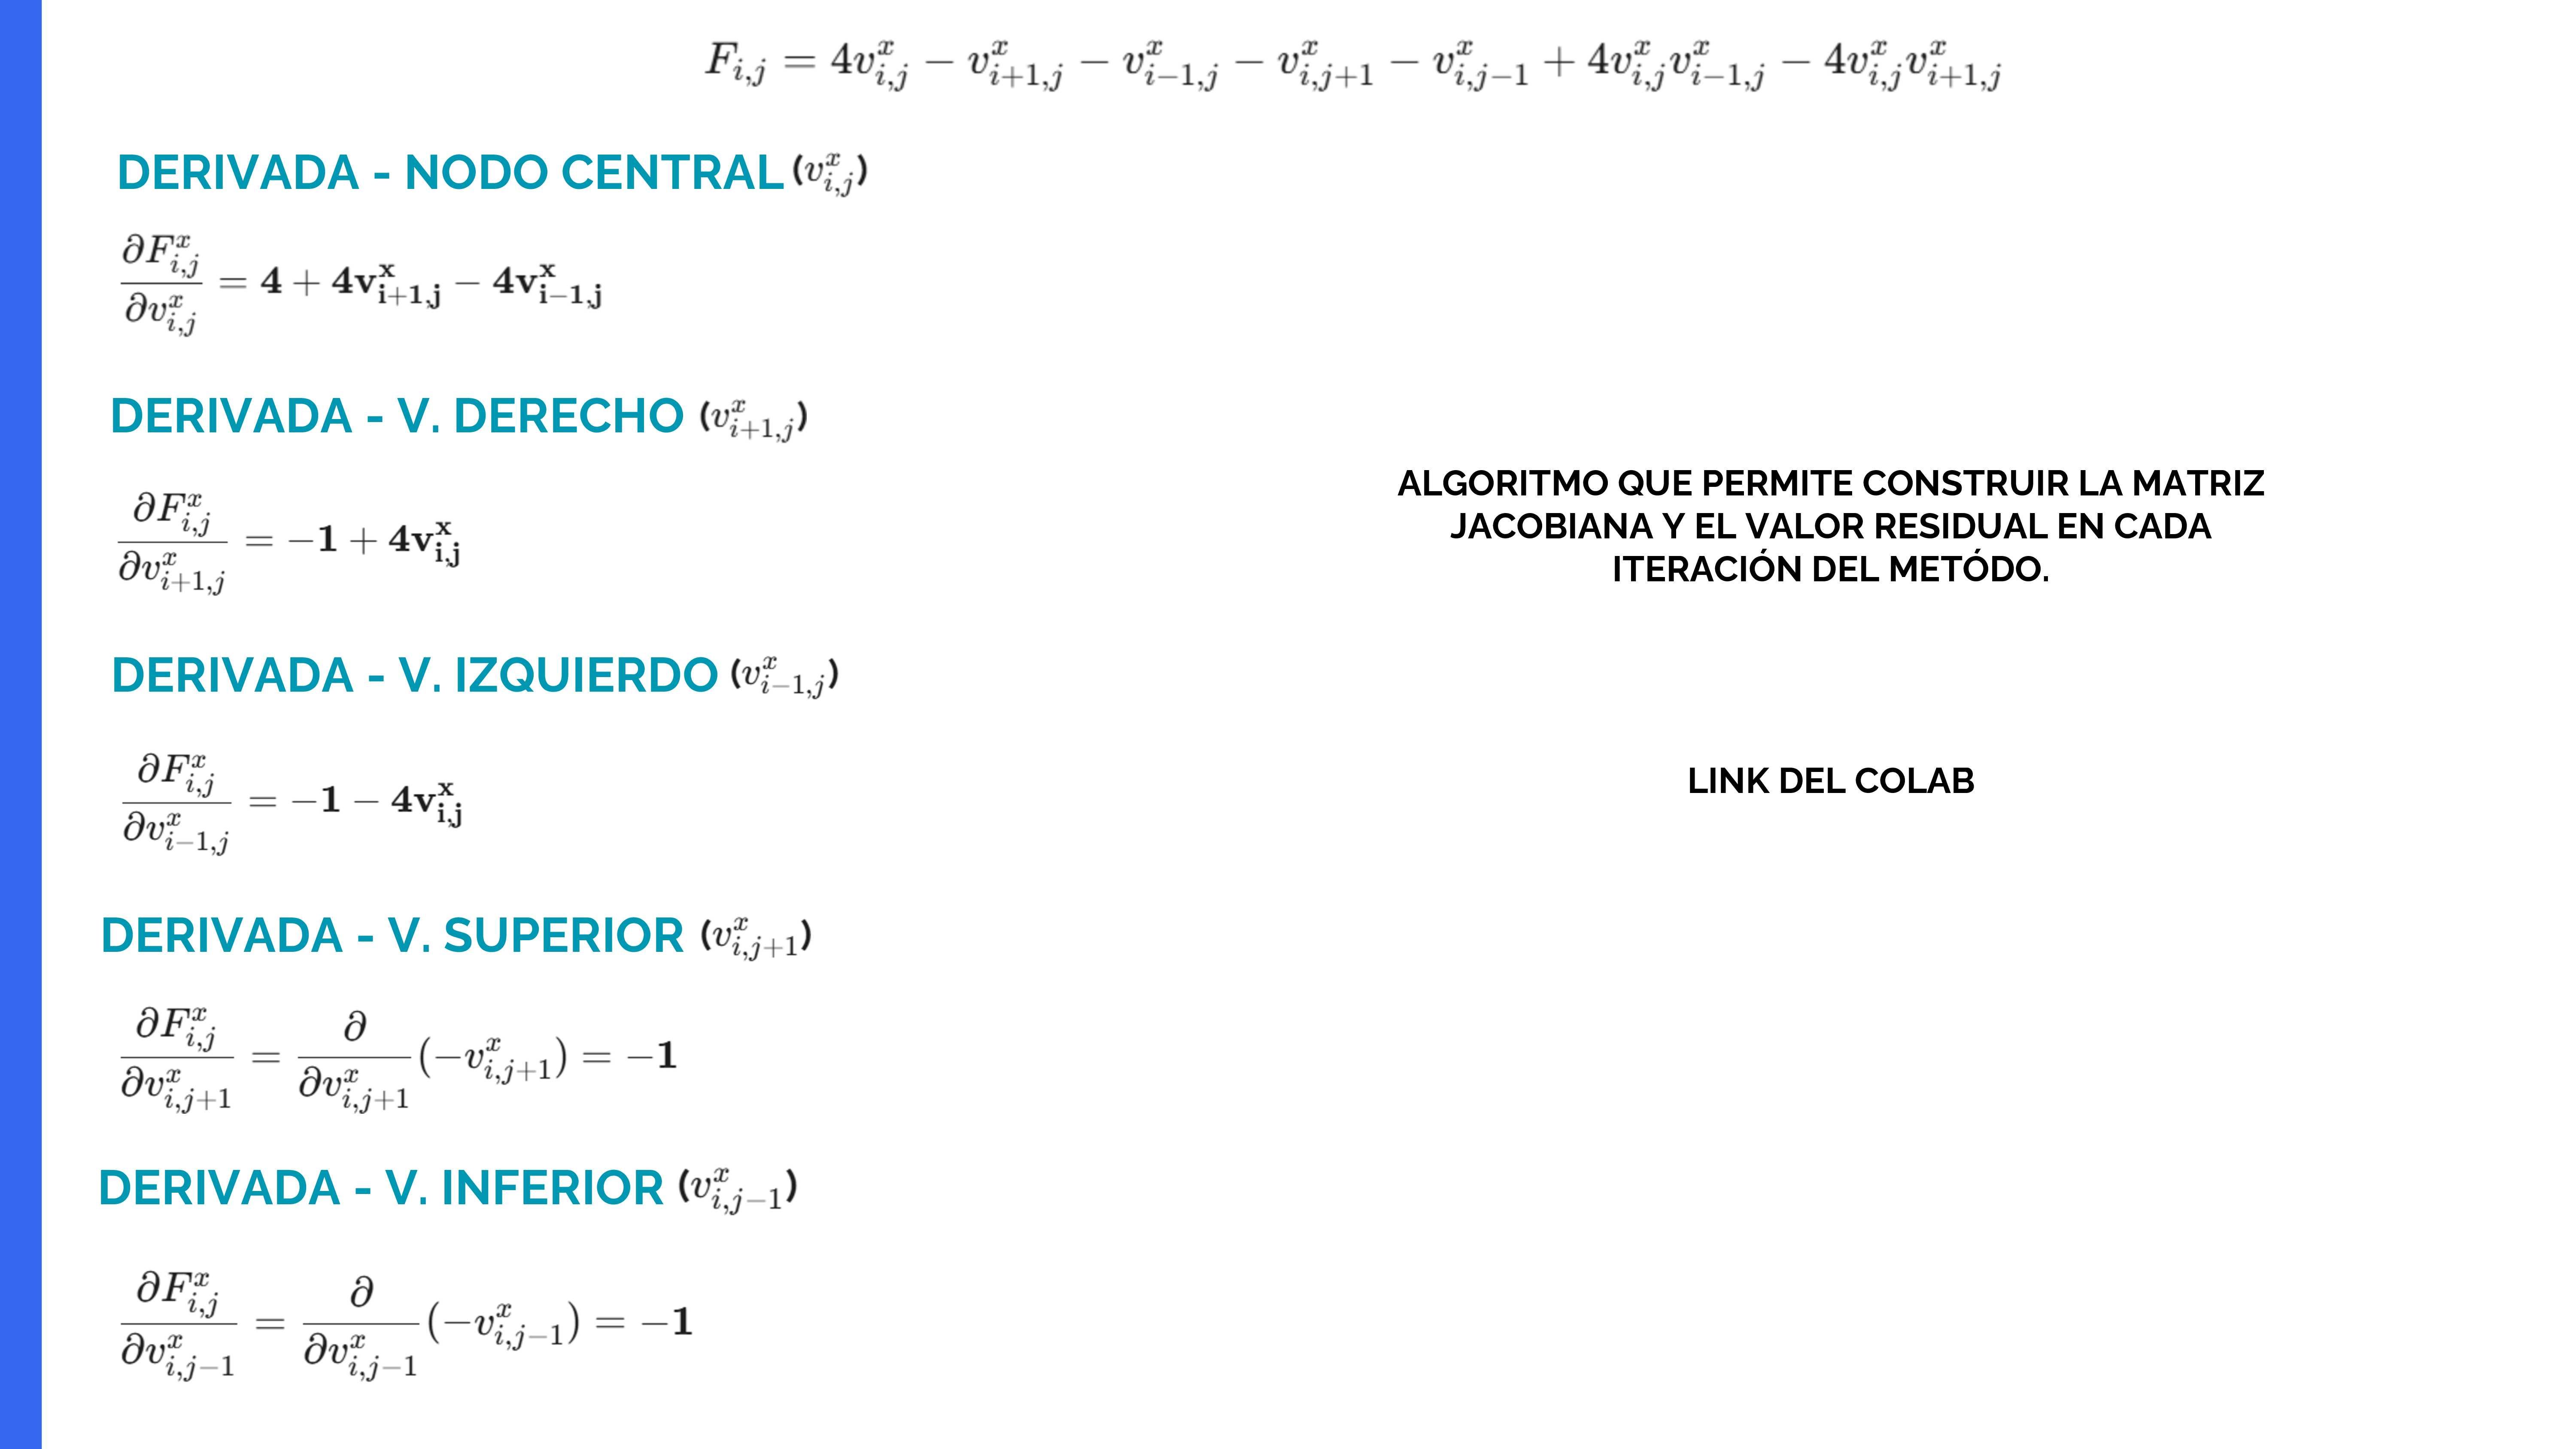
\includegraphics[width=0.95\textwidth]{intro_img-002.png}
  \caption{Derivadas parciales empleadas para el Jacobiano (extraída de `Introducción al sistema.pdf`).}
\end{figure}

\chapter{Algoritmo de Newton–Raphson}
Dado un estado \(V^{(k)}\):
\begin{enumerate}
  \item Ensamblar \(J(V^{(k)})\) y \(F(V^{(k)})\).
  \item Resolver el sistema lineal \(J\,\Delta V = -F\).
  \item Actualizar \(V^{(k+1)} = V^{(k)} + \Delta V\).
  \item Evaluar criterios de paro con \(\|F\|\) y/o \(\|\Delta V\|\).
\end{enumerate}
Equivalente en la notación del material: \(T(V^{(k)}) - A\,\Delta V^{(k)} = -F(V^{(k)})\), \(V^{(k+1)}=V^{(k)}+\Delta V^{(k)}\).

\begin{figure}[H]
  \centering
  
\includegraphics[width=0.95\textwidth]{intro_img-003.png}
  \caption{Esquema de NR y derivadas (extraída de `Introducción al sistema.pdf`).}
\end{figure}

\chapter{Implementación en Python (resumen)}
Se emplea \texttt{numpy} y \texttt{scipy.sparse}. A continuación se muestran extractos clave del código descrito en `AVANCE 2.md`/`AVANCE 2.docx`.

\section{Mapeo y acceso a valores}
\begin{lstlisting}[style=mypython,caption={Funciones de frontera, mapeo y acceso a V.}]
import numpy as np
from scipy.sparse import lil_matrix, linalg

# Parámetros de malla/condiciones
J_MAX = 3
I_MAX = 48
N_INCÓGNITAS = 134
V0 = 1.0
FACTOR_CONVECCION = 4.0

# Nodos de viga: (i in 20..29, j==1) fijos a 0

def get_velocidad_fija(i, j):
    if (j == 1 and i in range(20, 30)):
        return 0.0
    if j == 0:  # suelo
        return 0.0
    if j == 4:  # superficie G
        return V0
    if i == 0:  # entrada F
        return V0
    if i == 49: # salida H
        return 0.0
    return None

# Mapea (i,j) -> índice plano en [0, 133]; omite fronteras y viga

def map_to_index(i, j):
    if get_velocidad_fija(i, j) is not None:
        return -1
    base_index_j = 48 * (j - 1)
    index_i = i - 1
    desplazamiento_viga = 0
    if j == 1:
        if i >= 30:
            desplazamiento_viga = 10
        elif 20 <= i <= 29:
            return -1
    if j > 1:
        if j == 2:
            base_index_j = 38
        elif j == 3:
            base_index_j = 38 + 48
    final_index = base_index_j + index_i - desplazamiento_viga
    if final_index >= N_INCÓGNITAS or final_index < 0:
        return -1
    return final_index

def get_V_value(i, j, V_k):
    val_fijo = get_velocidad_fija(i, j)
    if val_fijo is not None:
        return val_fijo
    index = map_to_index(i, j)
    if index != -1:
        return V_k[index]
    return 0.0
\end{lstlisting}

\section{Ensamblaje de F y J}
\begin{lstlisting}[style=mypython,caption={Cálculo del residual F y el Jacobiano J.}]
def ensamblar_FJ(V_k):
    J = lil_matrix((N_INCÓGNITAS, N_INCÓGNITAS), dtype=np.float64)
    F = np.zeros(N_INCÓGNITAS)

    for j in range(1, J_MAX + 1):
        for i in range(1, I_MAX + 1):
            m = map_to_index(i, j)
            if m == -1:
                continue
            V_ij  = V_k[m]
            V_i1j = get_V_value(i + 1, j, V_k)
            V_im1j = get_V_value(i - 1, j, V_k)
            V_ij1 = get_V_value(i, j + 1, V_k)
            V_ijm1 = get_V_value(i, j - 1, V_k)

            F[m] = (4.0 * V_ij
                    - (V_i1j + V_im1j + V_ij1 + V_ijm1)
                    + (FACTOR_CONVECCION * V_ij * V_im1j)
                    - (FACTOR_CONVECCION * V_ij * V_i1j))

            J[m, m] = 4.0 + (FACTOR_CONVECCION * V_im1j) - (FACTOR_CONVECCION * V_i1j)
            n_der = map_to_index(i + 1, j)
            if n_der != -1:
                J[m, n_der] = -1.0 - (FACTOR_CONVECCION * V_ij)
            n_izq = map_to_index(i - 1, j)
            if n_izq != -1:
                J[m, n_izq] = -1.0 + (FACTOR_CONVECCION * V_ij)
            n_arr = map_to_index(i, j + 1)
            if n_arr != -1:
                J[m, n_arr] = -1.0
            n_aba = map_to_index(i, j - 1)
            if n_aba != -1:
                J[m, n_aba] = -1.0
    return J.tocsr(), F
\end{lstlisting}

\section{Ciclo de Newton–Raphson}
\begin{lstlisting}[style=mypython,caption={Iteraciones de Newton–Raphson.}]
def solve_newton_raphson():
    V_k = np.ones(N_INCÓGNITAS) * V0
    MAX_ITER = 100
    TOL = 1e-6
    for k in range(MAX
a_ITER):
        J_sp, F_vec = ensamblar_FJ(V_k)
        res_norm = np.linalg.norm(F_vec)
        if res_norm < TOL:
            break
        Delta_V = linalg.spsolve(J_sp, -F_vec)
        V_k += Delta_V
        if np.linalg.norm(Delta_V) < TOL:
            break
    return V_k
\end{lstlisting}

\paragraph{Notas de ejecución.} El solver resuelve un sistema lineal disperso por iteración. Es recomendable registrar \(\|F\|\) y \(\|\Delta V\|\) por iteración, y considerar estrategias de \emph{damping} en casos de no convergencia.

\chapter{Resultados esperados y discusión}
Se espera convergencia en un número moderado de iteraciones con inicialización razonable (p. ej. campo uniforme). El campo de solución \(V\) final puede proyectarse a la malla para su visualización (mapa de calor o contornos). Se recomienda validar derivadas del Jacobiano con diferencias finitas en algunos nodos y evaluar sensibilidad a tolerancias/condiciones de borde.

\chapter{Conclusiones}
El material del repositorio (\texttt{AVANCE 2.md}, \texttt{AVANCE 2.docx} y \texttt{Introducción al sistema.pdf}) presenta de forma coherente la formulación del método de Newton–Raphson para un sistema no lineal discretizado, el ensamblaje del Jacobiano y un esquema de implementación con \texttt{numpy}/\texttt{scipy.sparse}. Este informe integra dichas piezas en un formato académico con portada, ecuaciones, figuras y listados de código.

\chapter*{Referencias y archivos}
\begin{itemize}
  \item Documento visual: \texttt{Introducción al sistema.pdf} (figuras incluidas en este informe).
  \item Descripción detallada y código comentado: \texttt{AVANCE 2.md} y \texttt{AVANCE 2.docx}.
\end{itemize}

\end{document}
